\documentclass[10pt]{exam}
\usepackage[hon]{template-for-exam}
\usepackage{multicol,enumitem,tikz,multirow,fancybox}
\usetikzlibrary{shadings,decorations.pathmorphing,arrows.meta,patterns,calc}
\graphicspath{{./figures/}}
\title{Spring Lab}
\author{Rohrbach}
\date{\today}

\begin{document}
\maketitle

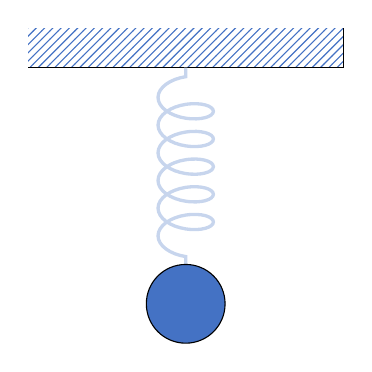
\begin{tikzpicture}
  \def\amp{3}
  \def\massradius{.5}
  \def\sep{2}
  \def\ceilingheight{1*\amp}
  \def\startofspring{\amp+1.5}
  \def\endofpicx{\startofspring+3.5*\sep}
  \def\springending{.1}
  \def\veclength{1.25}

  \definecolor{springcolor}{HTML}{4472C4}
  \definecolor{circlecolor}{HTML}{C5DFB5}

  \tikzstyle{guides}=[
      ultra thin,
      gray,
      dashed
    ]
  \tikzstyle{cmass}=[
      radius=\massradius,
      fill=circlecolor
    ]
  \tikzstyle{smass}=[
      radius=\massradius,
      fill=springcolor,
    ]
  \tikzstyle{ceiling}=[
      pattern=north east lines,
      pattern color=springcolor
    ]
  \tikzstyle{spring}=[
      very thick,
      springcolor!30,
      decoration={
        coil,
        amplitude=10
      }
    ]
  \tikzstyle{vector}=[
      red!30,
      very thick,
      ->
    ]

  \coordinate (ceiling start) 
                  at (-2, \ceilingheight);
  \coordinate (ceiling end)   
                  at (2, \ceilingheight);
  \fill[ceiling] (ceiling start) -- (ceiling end)
     -- ++(0,.5) -- ++ (-4,0) -- cycle;
  \draw (ceiling start) -- (ceiling end) -- ++ (0,.5);

  
  \path[smass] (0,0) coordinate (s3);


  %usage \drawspring{(location of mass)}{segment length}
  \newcommand{\drawspring}[2]{
    \coordinate (thismass) at #1;
    \coordinate (top) at 
      ($(ceiling start)!(thismass)!(ceiling end)$);
    \draw[spring,segment length=#2] (thismass)
      -- ++ (0,\massradius+\springending) 
      decorate {-- ($(top) + (0,-\springending)$) }
      -- (top);
  }


  \drawspring{(0,0)}{10}
  \draw[smass] (s3) circle;



\end{tikzpicture}

\paragraph{Purpose}
We are going to calculate the spring constant $k$ using two different methods.  If these two different methods give the same result, we will have confidence that our equations correspond to physical reality.

\paragraph{Ground Rules} \hfill
\begin{itemize}[topsep=0pt,itemsep=-1ex,partopsep=1ex,parsep=1ex]
  \item NEVER stretch the spring out with your hands
  \item NEVER place more than 200 grams on the spring
  \item When you are not actively taking measurements, do not leave masses hanging on the spring.
\end{itemize}

\section{Finding $k$ using Hooke’s Law}

In this experiment, we are going to measure how much different masses cause the spring to stretch and use this to determine spring constant.

\subsection*{Procedure}
\begin{enumerate}[topsep=0pt,itemsep=-1ex,partopsep=1ex,parsep=1ex]
  \item Without anything attached to the spring, record its height of the gram
  \item Place the 50-gram hangar on the spring and measure height off the ground (after the weight is on the spring).  Record in the chart
  \item Place different masses on the spring and measure the displacement.  \emph{Record in the chart.  Make sure all data is in m and kg.}
\end{enumerate}

\subsection*{Data}

\begin{tabular}{|c|c|c|}
  \hline
  \bf Total Mass & \bf Force applied to spring & \bf Height from the ground \\
  (hangar + mass) & ($W=mg$) &  \\
  (kg) & (N) & (m) \\\hline
  0 & & \\[1em]\hline
  0.050 & & \\[1em]\hline
  0.070 & & \\[1em]\hline
  0.100 & & \\[1em]\hline
  0.130 & & \\[1em]\hline
  0.150 & & \\[1em]\hline
  0.200 & & \\[1em]\hline

\end{tabular}

\subsection*{Analysis}
Make a graph on Desmos.  We are going to plot this a little bit backwards (and you will see why in a moment).  \textbf{Height should be $x$, Force should be $y$.}  Plot a best fit line.  Write down the equation for each of the best fit line below.  You should also copy the link to your graph, paste it on Schoology, and include the link here.


    \vspace{1em}

    Equation of Line:

    \vspace{2em}

    Link to graph: \texttt{https://www.desmos.com/calculator/}\fillin[][15em]


    \vspace{2em}

\noindent
Report your spring constant (with units) and then write a paragraph explaining what you did on this part of the lab.  Your paragraph should address: (1) What you graphed and what the graph looked like, (2) why the shape of the graph makes sense, and (3) how you used the graph to find your spring constant.

\vspace{1em}

Spring constant (with units): \fillin[][15em]

\vs


\begin{Sbox}\begin{minipage}{6.3in}
\subsection*{How to Graph on Desmos}

Go to \texttt{www.desmos.com/calculator} to graph your data. 

\begin{multicols}{2}

  \begin{enumerate}[label=\alph*),topsep=0pt,itemsep=-1ex,partopsep=1ex,parsep=1ex]
    \item \label{table} Start by making a table by clicking the “+” icon at the top left.  You will need to create two separate tables.
    \item \label{wrench} Make sure to label the axes using the wrench icon at the right.
    \item \label{zoom} Zoom out so that you can see the whole graph and so that it fills the page.  You can do this using the ``Zoom Fit'' option, but be careful that your fit does not cut off one of the graphs
    \item \label{linear} Create best fit lines for each graph using the ``Linear Regression'' tool
    \item Copy a link to your graph using the export button and clicking ``Share a Snapshot''.  Write down the link to this graph so you and your instructor can both access your work, later.
  \end{enumerate}

  \vspace{4em}

  \begin{tikzpicture}
    \node[anchor=north west] at (0,0) 
      {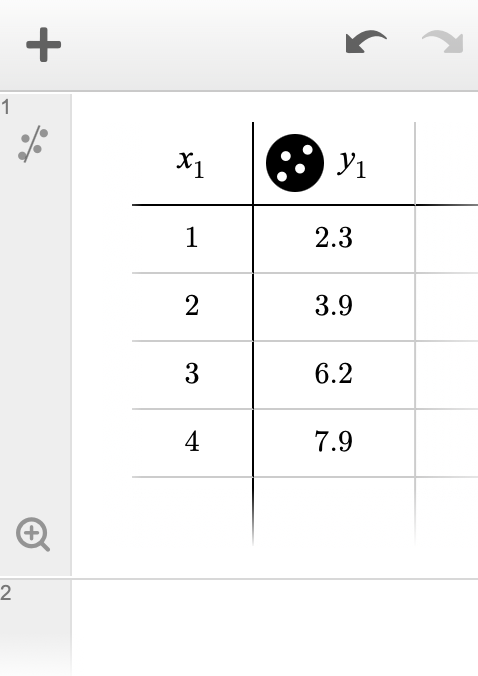
\includegraphics[width=3cm]{desmos1}};


    \node[anchor=north west] at (3.5,0) 
      {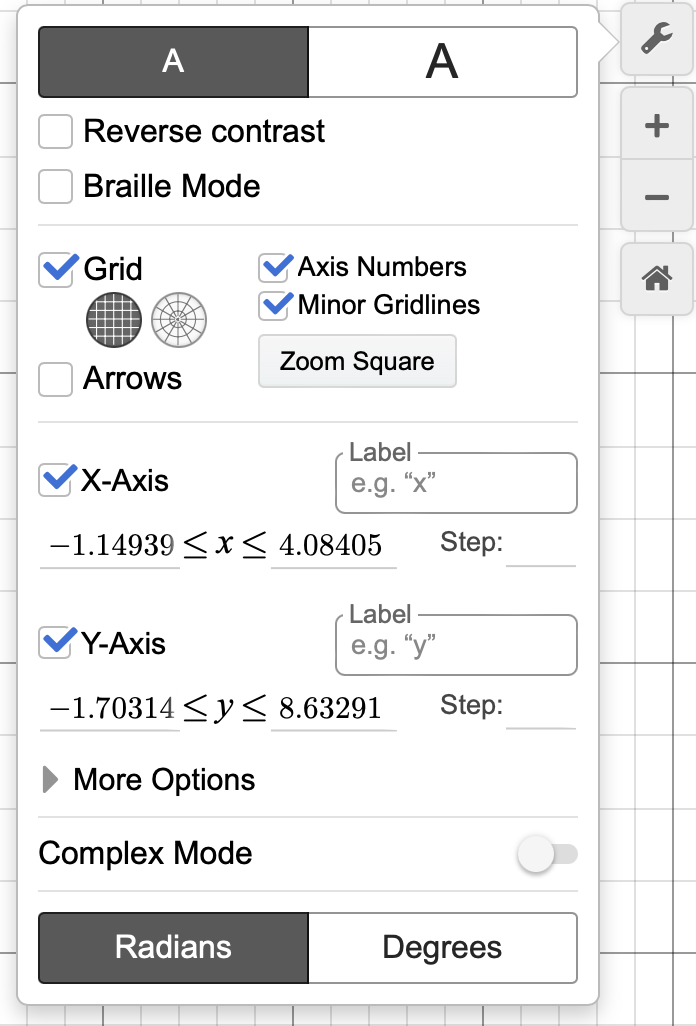
\includegraphics[width=3.5cm]{desmos2}};

        \draw (2,0) 
      node[fill=red!20,rounded corners] (table)
      {\ref{table} Create a table};
    \draw[red] (0.4,-.4) coordinate (a) circle (0.3);
    \draw[<-,red,very thick] (a) +(0.3,0) -- (table.south);

    \node[fill=blue!20,rounded corners] at (2.5,-1.5) (linear) {\ref{linear} Linear Regression};
    \draw[blue] (0.3,-1) coordinate (a) circle (0.3);
    \draw[<-,blue,very thick] (a) +(0.3,0) -- (linear.north);

    \node[fill=green!20,rounded corners] at (2,-2.5) (zoom) {\ref{zoom} Zoom Fit};
    \draw[green, ultra thick] (0.3,-3.5) coordinate (a) circle (0.3);
    \draw[<-,green,very thick] (a) +(0.3,0) -- (zoom.west);

    \node[fill=orange!20,rounded corners] at (4.5,-0.5) (wrench) {\ref{wrench} Axis Labels};
    \draw[orange, ultra thick] (6.9,-.3) coordinate (a) circle (0.3);
    \draw[<-,orange,very thick] (a) +(-0.3,0) -- (wrench.east);

    \draw[->,orange,very thick] (wrench.south) -- (5.2,-2.3);

    \draw[orange, ultra thick, rounded corners] (3.8,-2.3) rectangle ++(2.8,-0.5);
    \draw[orange, ultra thick, rounded corners] (3.8,-3.1) rectangle ++(2.8,-0.5);
  \end{tikzpicture}

\end{multicols}
\end{minipage}\end{Sbox}

\noindent
\shadowbox{\TheSbox}

\pagebreak
\section{Finding $k$ using the period of the spring}

In this experiment, we are going to measure the spring constant by looking at how the period of the spring varies with mass.

\subsection*{Procedure}
\begin{enumerate}[topsep=0pt,itemsep=-1ex,partopsep=1ex,parsep=1ex]
  \item Pick six different masses.  Make sure that they are evenly spread out and take full advantage of the amount of room the spring has to stretch.
  \item For each mass, set the spring in motion and measure the time of 5 oscillations.  Do this three times and take an average.
  \item Calculate the period and square it.
\end{enumerate}

\subsection*{Data}

  \def\cw{.11\textwidth}

  \begin{tabular}
    {
      |*{4}{>{\centering\bf\arraybackslash}m{\cw}|}
      >{\centering\arraybackslash}m{\cw}||>{\centering\arraybackslash}m{\cw}|>{\centering\arraybackslash}m{\cw}|
    }
    \hline
    \multirow{2}{\cw}
      {\centering \textbf{Mass $m$ (kg)}} & 
    \multicolumn{4}{c||}{\textbf{Time of 5 Oscillations (s)}}  & \multirow{2}{\cw}
      {\centering \textbf{Period $T$ (s)}} &
      \multirow{2}{\cw}{\centering \textbf{$T^2$ (s$^2$)}} \\
    \cline{2-5}
    & Trial \#1 & Trial \#2 & Trial \#3 & Average &&\\
    \hline
    &&&&&&\\[1em]
    \hline
    &&&&&&\\[1em]
    \hline
    &&&&&&\\[1em]
    \hline
    &&&&&&\\[1em]
    \hline
    &&&&&&\\[1em]
    \hline
    &&&&&&\\[1em]
    \hline
  \end{tabular}

  \subsection*{Analysis}
Make another graph on Desmos.  This time, \textbf{mass should be $x$ and $T^2$ should be $y$.}. Plot a best fit line.  Write down the equation for each of the best fit line below.  You should also copy the link to your graph, paste it on Schoology, and include the link here.




    \vspace{1em}

    Equation of Line:

    \vspace{2em}

    Link to graph: \texttt{https://www.desmos.com/calculator/}\fillin[][15em]


    \vspace{2em}

\noindent
Think about what the slope of your line represents.  It will be related to the spring constant.  To help you, take a look at the rearrangement of the frequency equation below
%
\begin{align}
  f &= \frac{1}{2\pi} \sqrt{\frac{k}{m}} \\
  \frac{1}{f} = T &= 2\pi \sqrt{\frac{m}{k}} \\
  T^2 &= \frac{4\pi^2 m}{k} \\
  T^2 &= \left(\frac{4\pi^2}{k}\right)m
\end{align} 
%

\noindent
Report your spring constant (with units) and then write a paragraph explaining what you did on this part of the lab.  Your paragraph should address: (1) What you graphed and what the graph looked like, (2) why the shape of the graph makes sense, and (3) how you used the graph to find your spring constant.  \emph{For part (3), Don't forget to explain why you did the calculation you did with the slope.}

\vspace{1em}

Spring constant (with units): \fillin[][15em]

\vs


\vspace*{\stretch{2}}
\section*{Conclusion}

In theory, both experiments should have yielded the same number for spring constant.  We are going to use the percent difference formula to determine how close your two numbers are.
%
\begin{align*}
  \text{Percent Difference} = \frac{\left| \text{measurement}_1 - \text{measurement}_2  \right|}{\text{avg. measurement}} \times 100\%
\end{align*}
%
Calculate the percent difference and then write a paragraph commenting on your percent error.  Your paragraph should address: (1) How reasonable is your percent error? (2) Identify three to four factors that could have created uncertainties in your measurements and explain how each factor may have influenced your percent error.


\vspace{1em}

Percent Difference: \fillin[][15em]

\vs[3]


\end{document}